\documentclass[xcolor=table]{beamer}
\usepackage{adjustbox}
\usepackage{comment}
\usetheme{Madrid}
\usepackage{wrapfig}


\title{Graph Neural Network Applications}

% A subtitle is optional and this may be deleted
\subtitle{Master in Innovation and Research in Informatics - Master's Thesis}

\author{Pau~Rodriguez}

\institute[]
{
  Universitat Politecnica de Catalunya\\
  MIRI - Data Science
  }

\date{October 2019}

\subject{}

\pgfdeclareimage[height=0.5cm]{./img/Logo_UPC}{./img/Logo_UPC}
\logo{\pgfuseimage{./img/Logo_UPC}}

\begin{comment}
\AtBeginSection[]
{
  \begin{frame}<beamer>{Outline}
    \tableofcontents[currentsection]
  \end{frame}
}
\end{comment}
\begin{comment}


\end{comment}

\begin{document}

\begin{frame}
  \titlepage
\end{frame}

\begin{frame}{Outline}
  \tableofcontents
\end{frame}



%------------------------------------------------------------------------
\section{Introduction}
\begin{frame}{Introduction}
    \begin{block}{What are Graph Neural Networks}
    {
     %Present a summarized view of Graph neural networks   
     %Present trends       
    }
    \end{block}

\end{frame}


%------------------------------------------------------------------------
\begin{frame}{Introduction}
    \begin{block}{What are Graph Neural Networks}
    {
    % Main papers and their applications in topics/areas list     
    }
    \end{block}

\end{frame}


%--------------------------------------------------------------------
\begin{frame}{Introduction}
    \begin{block}{Goals}
    {
     %The goal of this master’s thesis is to apply Graph Neural Network models to different problems to create a novel solution. The idea is to get to know how Graph Neural Networks are used in each situation. Two problems are explored: Girvan-Newmann algorithm approximation and compiled code function classification. They correspond to the two main tasks that Graph Neural Network perform with success, semi-supervised learning of nodes on a graph and supervised graph classification.        
    }
    \end{block}
    \begin{block}{Motivation}
    {
    % Graph Neural Networks seem to be a promising way of solving graph-related problems, with applications in many domains. The time seems right to jump into learning about the most recent models since they have attained state-of-the-art performance on some of the tasks they have solved.
    }
    \end{block}
\end{frame}

%------------------------------------------------------------------------
\begin{frame}{Introduction}
    \begin{block}{Organization}
    {
%      %The thesis is organized in the following way: the next section will explain the state-of-the-art in Graph Neural
% Network models by presenting the may models, their internals and the problems they have solved. Then, in
% section three, the methodology followed in the experiments is presented. After that, section four will go through
% an overview of the implementation of the experiments, whereas in section five the results of the experiments are
% summarized. Finally, in section six the conclusion of the thesis is presented.       
    }
    \end{block}
    
\end{frame}



%------------------------------------------------------------------------
\section{State of the art}
\begin{frame}{State of the art}{Nomenclature}
% summarize Notation subsection from SOTA on report G,V,E,...

\end{frame}



%------------------------------------------------------------------------
\begin{frame}{State of the art}{Euclidean space}
% Euclidean space definition
% why Graph are considered non Euclidean

%avoid??

\end{frame}




%------------------------------------------------------------------------
\begin{frame}{State of the art}{Graph Neural Networks}

% Graph Neural Network definitioin: Aggre, Combine, readout

% alternatives quick mention: hand-engineerred features, kernel funcs, markov-random walk embeddings

\end{frame}





%------------------------------------------------------------------------
\begin{frame}{State of the art}{Graph Neural Networks}


% Usual architecture: embedding + downstream ML algorithm


% tasks: node classif/regr, (sub)graph classif/regre 
%       -> repr. learning
% setupt: semi-supervised node repr. learning, and supervised graph repr. learning



\end{frame}




%------------------------------------------------------------------------
\begin{frame}{State of the art}{Graph Convolutional Networks}

% p6 sota GCN definition

% clarification: Kipf GCN versus broad type of convolutional networks
% convolution: sharing parameters


\end{frame}



%------------------------------------------------------------------------
\begin{frame}{State of the art}{Spectral methods}

% spectral methods characteristics pros and cons


\end{frame}


%------------------------------------------------------------------------
\begin{frame}{State of the art}{Spatial methods}
% spatial methods pros and cons
\end{frame}


%------------------------------------------------------------------------
\begin{frame}{State of the art}{Spatial methods - GCN}

%highlights 
%formula

\end{frame}


%------------------------------------------------------------------------
\begin{frame}{State of the art}{Spatial methods - MPNN}

%highlights 
%formula

\end{frame}


%------------------------------------------------------------------------
\begin{frame}{State of the art}{Spatial methods - GraphSage}

%highlights 
%formula

\end{frame}



%------------------------------------------------------------------------
\begin{frame}{State of the art}{Spatial methods - GGNN}

%highlights 
%formula

\end{frame}





%------------------------------------------------------------------------
\begin{frame}{State of the art}{Spatial methods - GIN}

%highlights 
%formula

\end{frame}


%------------------------------------------------------------------------
\begin{frame}{State of the art}{Other GNNs}

% G attention networks
% G AUto-encoders
% G Generative Networks
% G spatial-temporal networks
\end{frame}


%------------------------------------------------------------------------
\begin{frame}{State of the art}{Successful applications of GNN}

%CV
%Recsys
% BIochemistry
% Communication Networks modelling
% Program verification
\end{frame}



\section{Experiments}
%------------------------------------------------------------------------
\begin{frame}{Experiments}
    \begin{block}{General goal}{
    % Apply GNN to 2 experiments: one covering semi-supervised node regression(classification)
    % the other covering supervised graph classification in the domain :

    }\end{block}
    \begin{block}{General motivation}{
        % Make use of those great GNN algorithms in novel ways by applying them to new areas

    }\end{block}
    \begin{block}{Methodology}{
        % adaptation of CRIPS-DM without business understanding and deployment
        % for model selection & evaluation: hyper-parameter search with cross-validation for each type of model
        % types of models: from simple baselines to more complex ones
    }\end{block}



\end{frame}




%------------------------------------------------------------------------
\begin{frame}{Experiments}{Experiment 1 - Context}

% Girvan-newman algorithm

\end{frame}



%------------------------------------------------------------------------
\begin{frame}{Experiments}{Experiment 1 - Goals and motivation}

% Goal: find a novel way to approximate the GN algorithm

% motivation: community detection popular task 

\end{frame}


%------------------------------------------------------------------------
\begin{frame}{Experiments}{Experiment 1 - Description}

% what is done: semi-supervised node regression
%  switch to classification with ranges of edge betweenness values
% importance of the dataset split (nodes selection ) ->

\end{frame}


%------------------------------------------------------------------------
\begin{frame}{Experiments}{Experiment 1 - Results}


% table of results


\end{frame}

%------------------------------------------------------------------------
\begin{frame}{Experiments}{Experiment 1 - Conclusion}

% how good/bad is it?

% how it could be improved even more?



\end{frame}

%------------------------------------------------------------------------
\begin{frame}{Experiments}{Experiment 1 - Next steps}

% ways to apply this to Girvan-Newman approximation

\end{frame}



%------------------------------------------------------------------------
\begin{frame}{Experiments}{Experiment 2 - Context}

% papers that rename snippets of code or variables based on classification
Successful models for classifying code snippets or variables:  \cite{code2vec} , \cite{139}


% reverse engineering malicious code

% image of disassembled code

% explanation of the idea: rename function to help the analyst look faster for clues


\end{frame}


%------------------------------------------------------------------------
\begin{frame}{Experiments}{Experiment 2 - Context 2}

% reverse engineering malicious code
Reverse engineering malicious code (Computer virus)

% image of disassembled code:
%            ida pro free
%            a call to an unknown function 
%            code with comments on that call for example
%            function names and



% explain: compiled binary, 
% explain: assembler language, 
% explain: disassembler program,
% explain: reverse engineering malware (static analysis) = search for clues that help antivirus programs detect malicious code
%             like network communications, destination ip addresses,
%              destination domain names
%              files that are modified on the file system
%              mutexes (to avoid reinfection or multiple execution of the malicious code)


% explanation of the idea: rename function to help the analyst look faster for clues
Is it possible to rename the functions to help the analyst in searching specific functionalities within the code?

% arrow pointing the functions window

\end{frame}



%------------------------------------------------------------------------
\begin{frame}{Experiments}{Experiment 2 - Goals and Motivation}

\begin{block}{Goal}{
        }\end{block}
        % Goal classify snipets of assembler code (subroutines or functions)
        Classify snipets of assembler code (subroutines or functions) into well known general purpose functionalities (Network, Disk, Encryption,etc)

    }\end{block}
    \begin{block}{General motivation}{
        Speed up the process of reverse engineering malicious code by adding some indications on the main functionality of assembler functions.
    }\end{block}
\end{frame}


%------------------------------------------------------------------------
\begin{frame}{Experiments}{Experiment 2 - Description}

% data gathering

% data transformation

 

\end{frame}




%------------------------------------------------------------------------
\begin{frame}{Experiments}{Experiment 2 - Description 2}

% image of the final features of the dataset

% traininig

\end{frame}


%------------------------------------------------------------------------
\begin{frame}{Experiments}{Experiment 2 - Results}

% results table

\end{frame}

%------------------------------------------------------------------------
\begin{frame}{Experiments}{Experiment 2 - Conclusion}


% conclusion on why topological features don't give as much signal as code features
% features vs classes boxplots?



\end{frame}

%------------------------------------------------------------------------
\begin{frame}{Experiments}{Experiment 2 - Next steps}

% improvements

\end{frame}


\section{Conclusion}
%------------------------------------------------------------------------
\begin{frame}{Conclusion}{Results summary}

\end{frame}



%------------------------------------------------------------------------
\begin{frame}{Conclusion}{Next steps summary}

\end{frame}














% %-----------------------------------------------------------------------------------------------------------------------------------------------------------------------------------------------------------------------------

% \section{Multivariate Analysis}

% %------------------------------------------------------------------------------
% \begin{frame}{Multivariate Analysis}{Dataset}
% Our initial dataset: House sales in king county
% \begin{table}[H]
\centering
\resizebox{\textwidth}{!}{
\begin{tabular}{lll}
\hline
\rowcolor[HTML]{C0C0C0} 
id             & a notation for a house                                                                                                                                 & Numeric \\
date           & Date house was sold                                                                                                                                    & String  \\
\rowcolor[HTML]{C0C0C0} 
price          & Price is prediction target                                                                                                                             & Numeric \\
bedrooms       & Number of Bedrooms/House                                                                                                                               & Numeric \\
\rowcolor[HTML]{C0C0C0} 
bathrooms      & Number of bathrooms/bedrooms                                                                                                                           & Numeric \\
sqft\_living   & square footage of the home                                                                                                                             & Numeric \\
\rowcolor[HTML]{C0C0C0} 
sqft\_lot      & square footage of the lot                                                                                                                              & Numeric \\
floors         & Total floors (levels) in house                                                                                                                         & Numeric \\
\rowcolor[HTML]{C0C0C0} 
waterfront     & House which has a view to a waterfront                                                                                                                 & Numeric \\
view           & Has been viewed                                                                                                                                        & Numeric \\
\rowcolor[HTML]{C0C0C0} 
condition      & How good the condition is ( Overall )                                                                                                                  & Numeric \\
grade          & \begin{tabular}[c]{@{}l@{}}overall grade given to the housing unit, \\ based on King County grading system\end{tabular}                                & Numeric \\
\rowcolor[HTML]{C0C0C0} 
sqft\_above    & square footage of house apart from basement                                                                                                            & Numeric \\
sqft\_basement & square footage of the basement                                                                                                                         & Numeric \\
\rowcolor[HTML]{C0C0C0} 
yr\_built      & Built Year                                                                                                                                             & Numeric \\
yr\_renovated  & Year when house was renovated                                                                                                                          & Numeric \\
\rowcolor[HTML]{C0C0C0} 
zipcode        & zip                                                                                                                                                    & Numeric \\
lat            & Latitude coordinate                                                                                                                                    & Numeric \\
\rowcolor[HTML]{C0C0C0} 
long           & Longitude coordinate                                                                                                                                   & Numeric \\
sqft\_living15 & \begin{tabular}[c]{@{}l@{}}Living room area in 2015(implies-- some renovations) \\ This might or might not have affected the lotsize area\end{tabular} & Numeric \\
\rowcolor[HTML]{C0C0C0} 
sqft\_lot15    & lotSize area in 2015(implies-- some renovations)                                                                                                       & Numeric \\ \hline
\end{tabular}%
}
\caption{Dataset's features - House sales in king county}
\label{table:dataFeatures}
\end{table}
% \end{frame}


% %------------------------------------------------------------------------------
% \begin{frame}{Multivariate Analysis}{Preprocessing}
% \begin{itemize}
%     \item \textbf{Missing data and Errors - } The dataset is complete (no blanks\textbackslash Na's) 
%     \item \textbf{Outliers - } Using Robustified Mahalanobis distance, we remove 8 individuals 
% \end{itemize}

% \begin{figure}
% 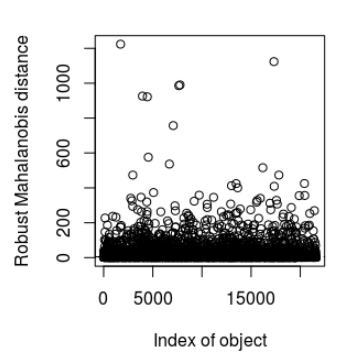
\includegraphics[scale=0.45]{./img/mahalanobis.png}
% \end{figure}

% \end{frame}


% %------------------------------------------------------------------------------
% \begin{frame}{Multivariate Analysis}{EDA: plots}

% \begin{figure}
% 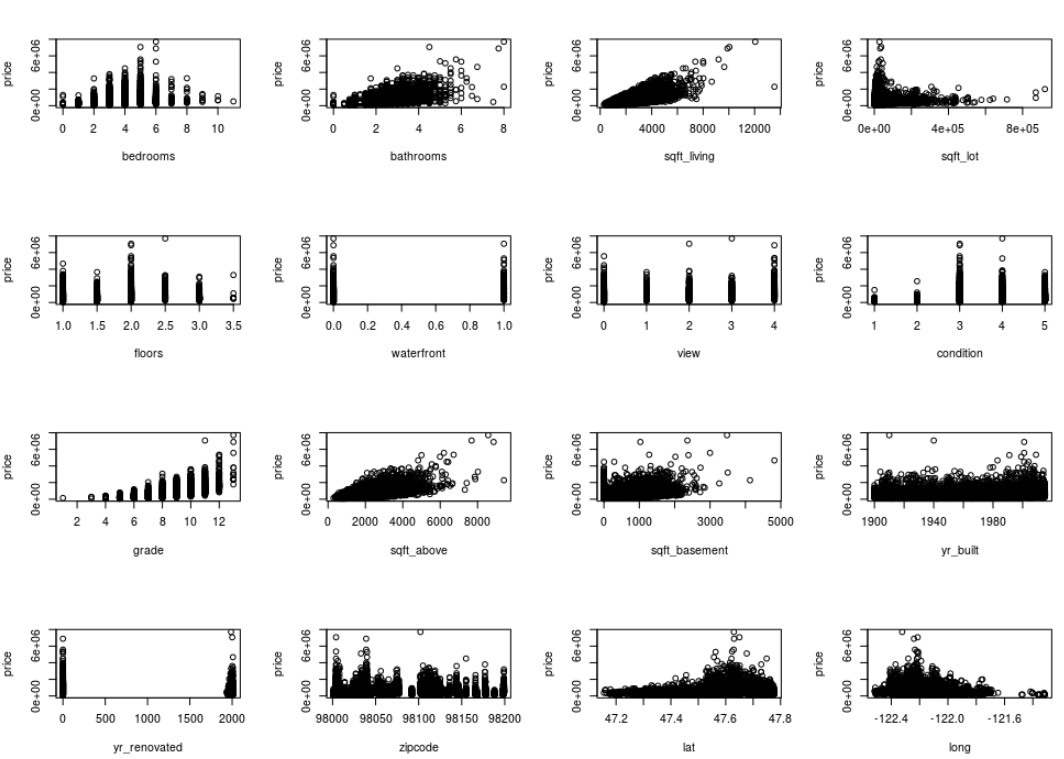
\includegraphics[scale=0.27]{./img/pairs-first.png}
% \end{figure}

% %We plot different variables of the dataset compared to the price, to start to graps what are the most important variables, what variables are possible candidates to be transformed.

% \end{frame}

% \begin{frame}{Multivariate Analysis}{EDA: histograms}

% \begin{figure}
% \includegraphics[scale=0.4]{./img/histograms.png}
% \end{figure}


% % we also plot histograms of each variables to see if they are drawn from a single distribution or not. etcetera
% \end{frame}


% %------------------------------------------------------------------------------
% \begin{frame}{Multivariate Analysis}{EDA: transformations}
% Logarithms and ratios
% \begin{figure}
% \includegraphics[scale=0.37]{./img/transformations.png}
% \end{figure}

% % here we have...
% %ratios capture same information in a lower dimension?
% %logs change the structure, correct skewness


% \end{frame}


% %------------------------------------------------------------------------------
% \begin{frame}{Multivariate Analysis}{EDA: transformations}
% Reducing skewness with logarithms.
% \begin{figure}
% \includegraphics[scale=0.32]{./img/log_skewness.png}
% \end{figure}

% %Logarithmic transformation can be useful to reduce skewness(for making patterns in the data more interpretable and for helping to meet the assumptions of inferential statistics). 
% % Not always worked so well.
% %>We also tried the Box-Cox transform, but didn't get better results than with this
% % we decided to create transformations for all continuous vars and then perform feature selection by experiments

% \end{frame}



% %------------------------------------------------------------------------------
% \begin{frame}{Multivariate Analysis}{EDA: correlation}
% For each highly correlated pair we remove one of the variables.
% \vspace*{-5pt}
% \begin{figure}
% 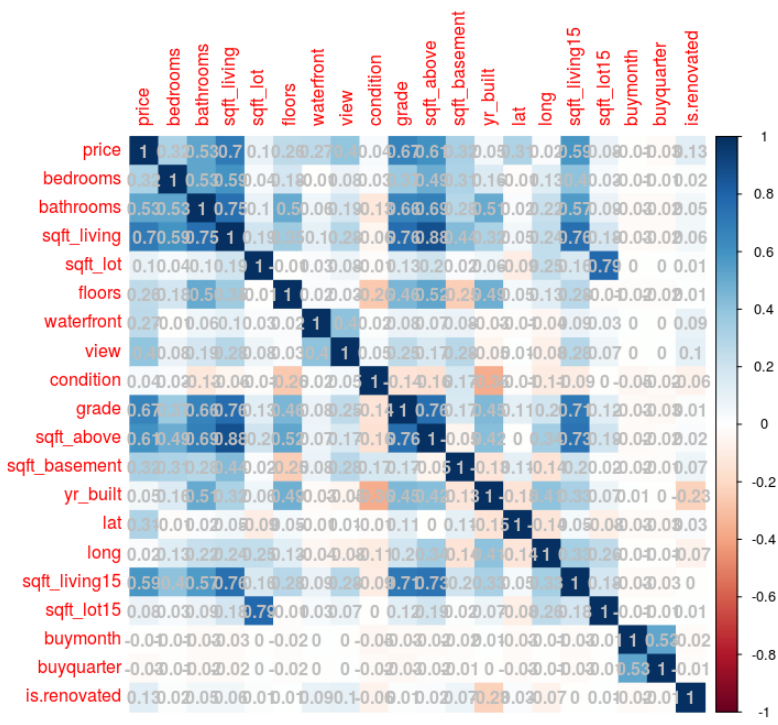
\includegraphics[scale=0.27]{./img/corr01.png}
% \end{figure}
% %\vspace*{-35pt}
% %we transform the variables using logarithms and ratios. sqft_living log transformation, bedroom/floor, floor/bathrooms, bathrooms/bedrooms = which can give an idea of the amount of money spent on the house, logarithm transform som echange of aspect.

% \end{frame}


% %------------------------------------------------------------------------------
% \begin{frame}{Multivariate Analysis}{EDA: correlation}
% For each highly correlated pair we remove one of the variables.
% \vspace*{-5pt}
% \begin{figure}
% \includegraphics[scale=0.27]{./img/corr02.png}
% \end{figure}
% %\vspace*{-35pt}
% % sqft_lot15/sqft_lot15, sqft_living15/sqft_living, sqft_above/sqft_living
% \end{frame}


% %------------------------------------------------------------------------------
% \begin{frame}{Multivariate Analysis}{EDA: correlation}
% For each highly correlated pair we remove one of the variables.
% \vspace*{-5pt}
% \begin{figure}
% \includegraphics[scale=0.25]{./img/corr03.png}
% \end{figure}
% %\vspace*{-35pt}

% \end{frame}



% %------------------------------------------------------------------------------
% \begin{frame}{Multivariate Analysis}{Unsupervised analysis: PCA}
% Correlations between variables and target(Price)
% \vspace*{-8pt}
% \begin{figure}
% 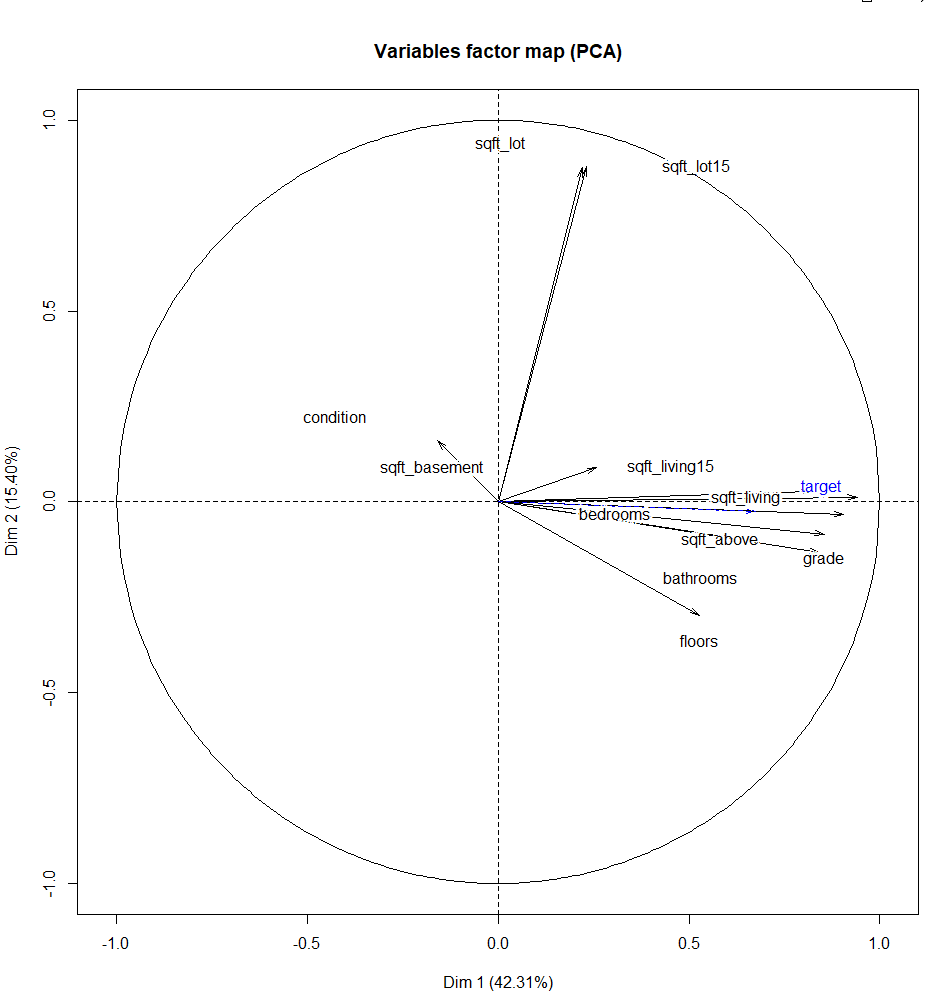
\includegraphics[scale=0.34]{./img/PCA.png}
% \end{figure}
% %sqft_lot not correlated (almost orthogonal)
% %the rest of continuous variables (sqft_living, bedrroms, sqft_above, grade, bathrroms) highly correlated between them and with the price
% % correlation between predictor variables is generally bad for training the models

% \end{frame}



% %------------------------------------------------------------------------------
% \begin{frame}{Multivariate Analysis}{Unsupervised analysis: Hierarchical Clustering}

% Assumption: only one cluster
% \begin{figure}
% 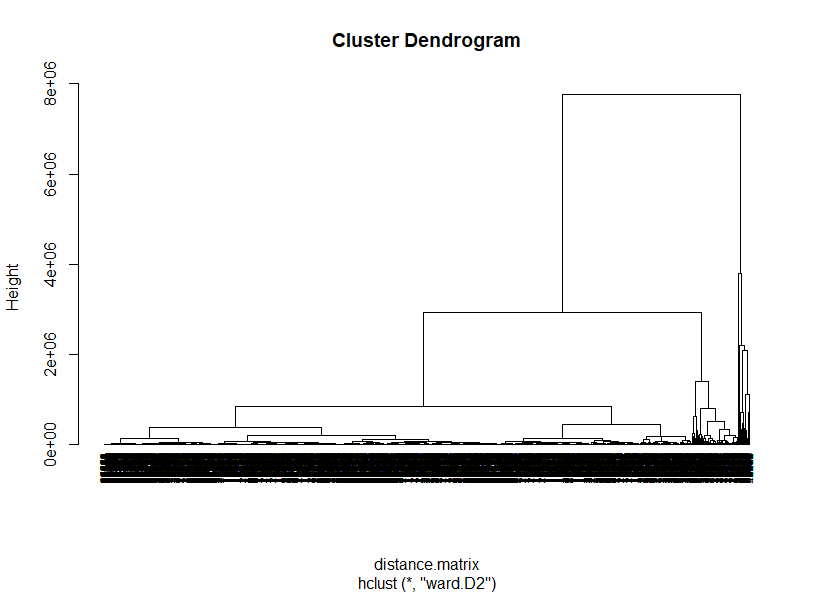
\includegraphics[scale=0.4]{./img/Hclustering.png}
% \end{figure}
% % worried about if there are different clusters for the data
% % after performing a hierarchycal clustering we conclude we can assume only one cluster
% % other wise, we would be forced to train different models for each cluster, and separate train and testing data according to the proximity to the centroid of each of the clusters.

% \end{frame}

% %Feature extraction
% %Feature extraction - logs, ratios: which ones
% %Feature extraction - correlation : the subsets we select 
% %Feature extraction - PCA  -> how we build the features + target


% \section{Feature Extraction}
% %------------------------------------------------------------------------------
% \begin{frame}{Feature Extraction}
% For each transformation: 
% \begin{itemize}
%     \item logarithms
%     \item ratios
%     \item removing highly correlated variables
%     \item significant principal components from PCA
% \end{itemize}
% we create new datasets by binding the new variables with the original target variable.

% \end{frame}


% %------------------------------------------------------------------------------
% \begin{frame}{Feature Extraction}
% Derived datasets:
% \input{./tables/datasets.tex}

% \end{frame}


% %models
% %Models - methodology
% %Models - selected models (maybe in one single slide all of them!)
% %Models - selected models - linear
% %Models - selected models - Ridge regression
% %Models - selected models - Lasso regression
% %Models - selected models - Decision trees for regression
% %Models - selected models - Random Forest for regression
% \section{Models}
% %------------------------------------------------------------------------------
% \begin{frame}{Models}{Methodology}

% Common training model methodology:
% \begin{itemize}
%     \item \textbf{Split dataset:} randomly split the training and test dataset 
%     \item \textbf{Model selection:}model selection(hyperparameters) by cross validation over the training set
%     \item \textbf{Refit:} refit of the model over all the training set with selected hyper parameters
%     \item \textbf{Generalization:} prediction of the model over test set to compute the testing error
% \end{itemize}
% We use the NRMSE.

% \end{frame}


% %------------------------------------------------------------------------------
% \begin{frame}{Models}{Methodology}

% Selected types of models:
% \begin{itemize}
%     \item Linear regression
%     \item Ridge regression
%     \item Lasso regression
%     \item Decision trees
%     \item Random forest
% \end{itemize}

% \end{frame}

% %Experiments
% %Experiments - overview
% %Experiments - initial exploration
% %Experiments - Feature selection
% %Experiments - Refinement
% %Experiments - Results
% \section{Experiments}
% %------------------------------------------------------------------------------
% \begin{frame}{Experiments \& Results}{Methodology overview}
% Our approach consists on exploration with final refinement:
% \begin{enumerate}
%     \item \textbf{Space exploration - }train all models, each with all the generated datasets and select the best 3.
%     \item \textbf{Feature selection - }for each model and dataset,
%     \item \textbf{Refit - }refit the best 3 models after feature selection.
% \end{enumerate}

% \end{frame}

% %------------------------------------------------------------------------------
% \begin{frame}{Experiments \& Results}{Space exploration}
% \vspace*{-5pt}
% Fragment of the experiments during exploration
% \vspace*{2pt}
% \input{./tables/exp_models_vs_featuresets_presentation.tex}
% \end{frame}

% %------------------------------------------------------------------------------
% \begin{frame}{Experiments \& Results}{Space exploration}
% Sorted plot of the validation, training and testing error (NRMSE)
% \vspace*{-7pt}
% \begin{figure}
% 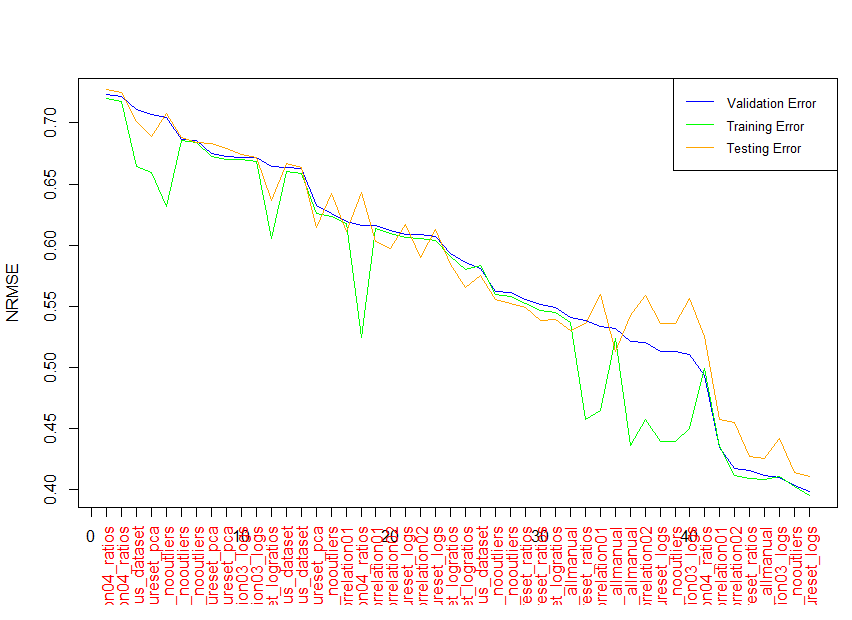
\includegraphics[scale=0.5]{./img/exp01.png}
% \end{figure}
% \end{frame}


% %------------------------------------------------------------------------------
% \begin{frame}{Experiments \& Results}{Space exploration}
% Selected models and datasets 
% \vspace*{3pt}
% % latex table generated in R 3.4.3 by xtable 1.8-2 package
% 
\begin{table}[H]
\begin{tabular}{cllcc}
  \hline
 & Model & Dataset & Validation NRMSE & Testing NRMSE \\ 
  \hline
  51 & regression\_randomforest & featureset\_logs & 0.40 & 0.41 \\ 
  42 & regression\_tree\_rpartlib & featureset\_nocorrelation03\_logs & 0.51 & 0.56 \\ 
  25 & lasso regression GLMNET & featureset\_allmanual & 0.53 & 0.51 \\ 
  
   \hline
\end{tabular}
\label{experiments}\caption{Experiments performed and their NRMSE for validation and testing }
\end{table}

% \end{frame}


% %------------------------------------------------------------------------------
% \begin{frame}{Experiments \& Results}{Feature selection}

% Evolution of the validation error in the Backward selection algorithm execution for the Lasso model. We had a minor improvement but in the end the dataset was smaller.
% \vspace*{-7pt}
% \begin{figure}
% \includegraphics[scale=0.3]{./img/lasso_SBS.png}
% \end{figure}

% \end{frame}


% %------------------------------------------------------------------------------
% \begin{frame}{Experiments \& Results}{Feature selection}

% Evolution of the validation error in the Backward selection algorithm execution for the Random Forest model.
% We can see that removing latitude or longitude has negative impact on the validation error whereas removing sqrt\_lot will reduce the validation error in 1\%.
% \vspace*{-7pt}
% \begin{figure}
% \includegraphics[scale=0.3]{./img/SBS.png}
% \end{figure}

% \end{frame}


% %------------------------------------------------------------------------------
% \begin{frame}{Experiments \& Results}{Refit \& Result}

% Final result
% \vspace*{3pt}
% \begin{table}[H]
\centering
\resizebox{\textwidth}{!}{
\begin{tabular}{cllccc}
  \hline
 & Model & Feature set & Validation.NRMSE & Training.NRMSE & Testing.NRMSE \\ 
  \hline
1 & regression\_tree\_rpartlib & featureset\_regression\_rpart\_tree\_fitting\_sfs & 0.51 & 0.45 & 0.56 \\ 
  2 & lasso regression GLMNET & featureset\_glmnet\_lasso\_sfs & 0.54 & 0.53 & 0.52 \\ 
  3 & regression\_randomforest & featureset\_regression\_randomforest\_sfs & 0.59 & 0.59 & 0.59 \\ 
   \hline
\end{tabular}
}
\caption{Best 3 models}
\label{table:final}
\end{table}
% \end{frame}



% %Conclusion
% %Conclusion - Presenting results
% %Conclusion - comparison of models/algorithms
% %Conclusion - Final impressions
% \section{Conclusion}
% %------------------------------------------------------------------------------
% %\begin{frame}{Conclusion}
% %    \begin{block}{\center Million dollar question}
% %    \center What is the best combination of feature set and model? 
% %    \end{block}
% %    \begin{block}{}
% %    Sequential forward selection performance:
% %    \begin{itemize}
% %        \item Choose sub-optimal feature set for random forest $\rightarrow$ that led to higher validation error.
% %        \item Decision trees and Lasso regression are less sensitive and SFS choose good feature set that preforms as good as found by exploration.
% %    \end{itemize}
% %    \end{block}
% %    \begin{block}{}
% %    During exploration RF overcome all other models. However, with SFS the generated forests under-preformed even compared to the decisions tree. 
% %    \end{block}
% %\end{frame}


% \begin{frame}{Conclusion}
%     \begin{block}{\center Million dollar question}
%     \center What is the best combination of feature set and model? 
%     \end{block}
%     \begin{block}{}
%     Sequential Backward selection performance:
%     \begin{itemize}
%         \item Random forest preformed better with smaller subset.
%         \item Decision trees and Lasso regression are less sensitive and SBS choose good feature set that preforms as good as found by exploration.
%     \end{itemize}
%     \end{block}
%     \begin{block}{}
%     During exploration RF overcome all other models and got even better performance using SBS.
%     Trying to use SFS, the generated RF under-preformed even compared to the decisions tree, it happens because the SFS lead to local minimum. 
%     \end{block}
% \end{frame}

% %------------------------------------------------------------------------------
% %\begin{frame}{Conclusion}
% %    \begin{block}{\center why?}
% %    What is the best combination of feature set and model? 
% %    \begin{itemize}
% %        \item  Random forest expected to be the best model $\rightarrow$ but highly dependent on the dataset.
% %        \item Decision trees and Lasso regression are less sensitive to the dataset.
% %    \end{itemize}
% %    \end{block}

% %\end{frame}

% %------------------------------------------------------------------------------
% \begin{frame}{Conclusion}{Future work}
% \begin{block}{Proposed improvements}
% \begin{itemize}
%     \item Test more advanced models: Splines, RVM, Bayesian approach to regression
%     \item Perform a deeper exploration of the possible features and combinations of features
%     \item Explore better feature selection methods: Bi-directional search, Plus-L Minus-R selection etc.
% \end{itemize}
% \end{block}
% \end{frame}

\end{document}


